
\subsection{Simulation method}

This part will analyze the effect of several parameters on 3 aspects of the result, which is the probability of creating barrier, the average coverage of the multiple view sensor barrier and the overall computational time. The algorithm is performed on every instance and keep recording 3 data, the creation of barrier, the computational time and the exposure on a barrier if there is one. Then, the result are combined for all instances of the same parameter settings to achieve the probability of barrier creation, the average computational time and the average exposure value on the found barriers.

\subsection{System setting and parameters setting}
%Đoạn này hư cấu sửa sau :v
System settings

All the experiments are performed on a personal computer with core Intel Core i7-7700HQ, 8GB of DDR4 RAM running on Windows 10 Home, the programming language used to simulate the algorithm is Java 11.

Parameter settings

The sensing fields in all experiments are presented as rectangles with the size of 200m x 50m. Sensor nodes are deployed uniformly in a rectangle with each side extended compared to the sides of the sensing field a distance equal to the sensing radius of each sensor in order to guarantee the uniform distribution regarding sensing area inside the sensing field. Each set of parameters contains several independent random topologies to conduct the algorithm on and measure the target indexes. Furthermore, each instance of experiment is conducted with both node handling methods. Altogether there are 42000 experiments on 210 instances of parameters which were analyzed with our algorithm. The details are as follows:
\begin{table}[h!]
	\centering
	\begin{tabular}{l | r}
		Length & 200 \\
		Width & 50 \\
		Sensing Radius & 30 \\
		Minimum sensing radius & 5 \\
		Sensing angle & 90 \\
		k & 3, 4, 5, 6 \\
		The number of topologies for each instance & 100 \\
		Node handling method & Max, Random
		
	\end{tabular}
	\caption{General parameters}
\end{table}

\begin{table}[h!]
	\centering
	\begin{tabular}{l | c | c | c | c}
		k & 3 & 4 & 5 & 6\\
		$\omega$ & 90 - 115 & 55 - 80 & 40 - 60 & 35 - 50\\
	\end{tabular}
	\caption{Problem parameters}
\end{table}

\subsection{Computation results}

\subsubsection{Effect of $\omega$ on algorithm performance}

$\omega$ is an important parameter in the $k-\omega$ coverage model. As a result, this parameter has a considerable impact on the output of the algorithm. Because $\omega$ is a lower bound for the angle between two consecutive sensors in the perspective of the considered point, every sensor set that satisfies the condition with large $\omega$ would also successfully make a $k-\omega$ cover with lower $\omega$. In short, a decrease in parameter $\omega$ may result in an expansion in the result space of the algorithm. This leads to two different consequences. On the one hand, there would be more sets of sensor $k-\omega$ cover a single node, which means that the coverage value of that node is likely to be lifted. However, on the other hand, the lower value of $\omega$ could reduce the average rank of the covered nodes, as the nodes are more easily covered, which leads to a lower coverage value, since the sets that cover the bigger node tend to position further than the sets covering the smaller ones.

As a consequence, firstly, with a lower value of $\omega$, the algorithm would offer a greater chance of $(k-\omega)$ barrier existence. However, the probability of forming barriers can never exceed $100\%$, the curve that represents the barrier probability would approach $100\%$ and does not rise higher with lower $\omega$. Regarding coverage value, while the max method illustrate an downward trend, the random method tends to go up while the value of $\omega$ keep rising. This result is not applied to very large value of $\omega$, where the low barrier probability leads to little number of examined sensing field, which results in a high variance and the obtained results would be less concrete. However, despite overall trends, the coverage value obtained with different $\omega$ is observed not to change significantly, and the difference can be accepted in real circumstances.

Finally, a lower value of $\omega$ results in a larger searching space, which leads to a drastic rise in computation time to conduct the max method, while the random method does not suffer from this property. This result may come from the fact that the max method require the evaluation of the coverage value of every $(k-\omega)$ sensor list toward each node, which seems to be an exception job.

\begin{figure}[h]
	\begin{subfigure}[t]{.5\textwidth}
		\centering
		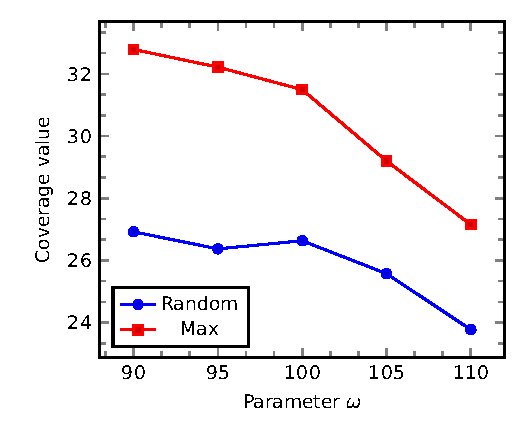
\includegraphics[scale=.8]{Hinhanh/OmegaEffect/coverage/k3.pdf}
		\caption{k = 3}
	\end{subfigure}
%	\hfill
	\begin{subfigure}[t]{.5\textwidth}
		\centering
		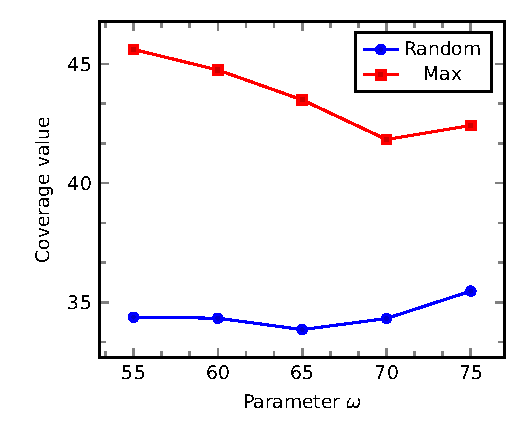
\includegraphics[scale=.8]{Hinhanh/OmegaEffect/coverage/k4.pdf}		
		\caption{k = 4}
	\end{subfigure}
\caption{Effect of $\omega$ on the average coverage value of the found barrier with $k = 3$ and $k = 4$}
\label{fig:}
\end{figure}
%
\begin{figure}[h]
	\begin{subfigure}[t]{.5\textwidth}
		\centering
		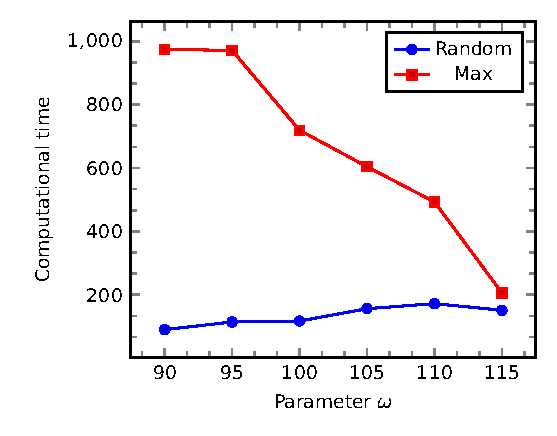
\includegraphics[scale=.8]{Hinhanh/OmegaEffect/time/k3.pdf}		
		\caption{k = 3}
	\end{subfigure}
	\begin{subfigure}[t]{.5\textwidth}
		\centering
		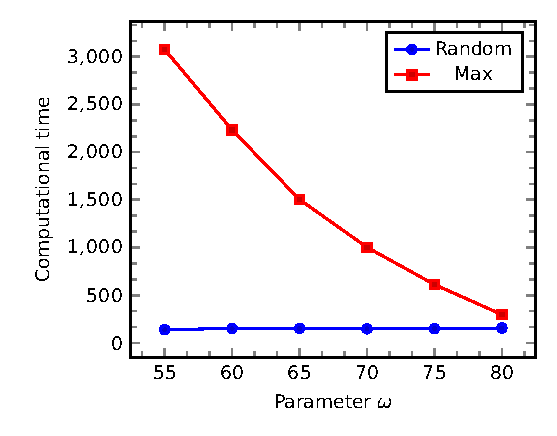
\includegraphics[scale=.8]{Hinhanh/OmegaEffect/time/k4.pdf}		
		\caption{k = 4}
	\end{subfigure}
\caption{Effect of $\omega$ on the average computational time in $ms$ of the algorithm with $k = 3$ and $k = 4$}
\label{fig:}
\end{figure}
%
\begin{figure}[h]
	\begin{subfigure}[t]{.5\textwidth}
		\centering
		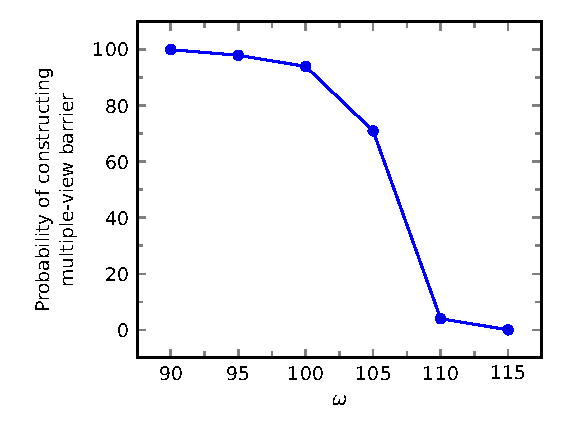
\includegraphics[scale=.8]{Hinhanh/OmegaEffect/probability/k3.pdf}		
		\caption{k = 3}
	\end{subfigure}
	\begin{subfigure}[t]{.5\textwidth}
		\centering
		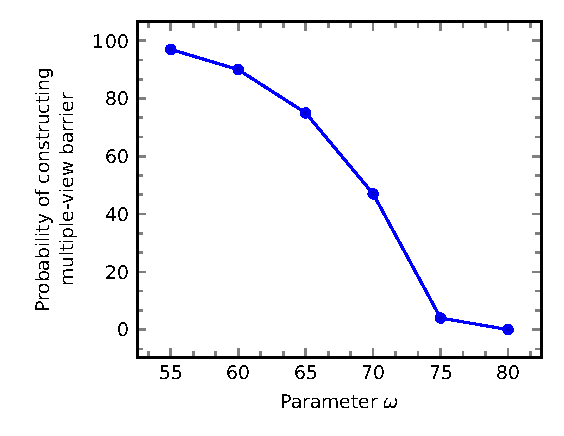
\includegraphics[scale=.8]{Hinhanh/OmegaEffect/probability/k4.pdf}		
		\caption{k = 4}
	\end{subfigure}
\caption{Effect of $\omega$ on the probability of existence of multiple view barrier with $k = 3$ and $k = 4$}
\label{fig:}
\end{figure}

\subsubsection{Effect of sensor number on algorithm performance}

Similar to the effect of $\omega$, a larger value of sensor number would lead to a larger searching space. However, in this occasion, the negative effect on coverage value seems to be more significant. As a result, the barrier coverage value tends to fall slowly as the sensor number rises for both node handling methods. Furthermore, the large number of sensors leads to a huge computational work, as the time required to run both methods rise linearly with the increase of the sensor number. This results in the computation time surge dramatically as the sensor number grows.

\begin{figure}[h]
	\begin{subfigure}{.5\textwidth}
		\centering
		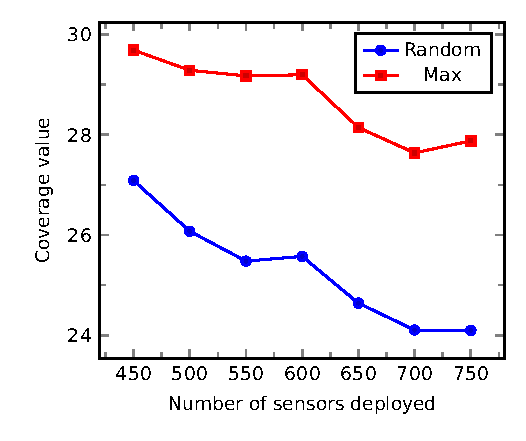
\includegraphics[scale=.8]{Hinhanh/SensorNumberEffect/coverage/k3omega105.pdf}
		\caption{k = 3, $\omega$ = 105}
	\end{subfigure}
	\begin{subfigure}{.5\textwidth}
		\centering
		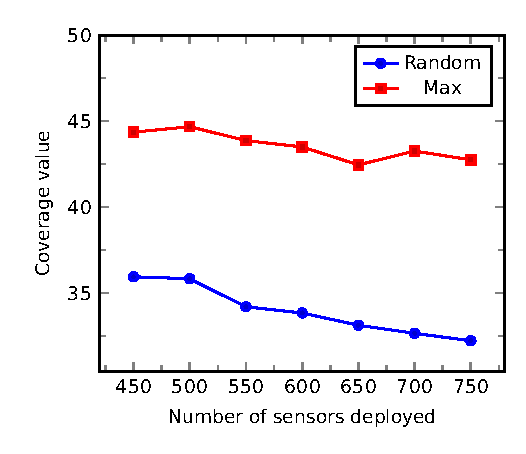
\includegraphics[scale=.8]{Hinhanh/SensorNumberEffect/coverage/k4omega65.pdf}
		\caption{k = 4, $\omega$ = 65}
	\end{subfigure}
\caption{Effect of sensor number on the average coverage value of the found barrier with some typical values of $k$ and $\omega$}
\label{fig:}
\end{figure}
%
\begin{figure}[h]
	\begin{subfigure}{.5\textwidth}
		\centering
		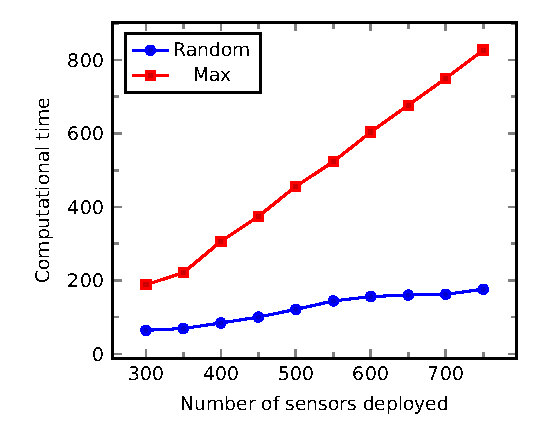
\includegraphics[scale=.8]{Hinhanh/SensorNumberEffect/time/k3omega105.pdf}
		\caption{k = 3, $\omega$ = 105}
	\end{subfigure}
	\begin{subfigure}{.5\textwidth}
		\centering
		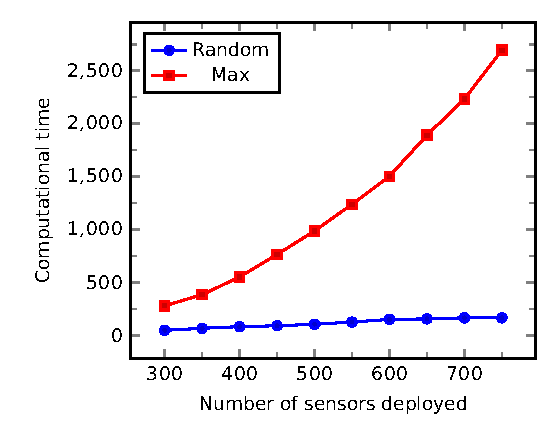
\includegraphics[scale=.8]{Hinhanh/SensorNumberEffect/time/k4omega65.pdf}
		\caption{k = 4, $\omega$ = 65}
	\end{subfigure}
\caption{Effect of sensor number on the average computational time in $ms$ of the algorithm with some typical values of $k$ and $\omega$}
\label{fig:}
\end{figure}
%
\begin{figure}[h]
	\begin{subfigure}{.5\textwidth}
		\centering
		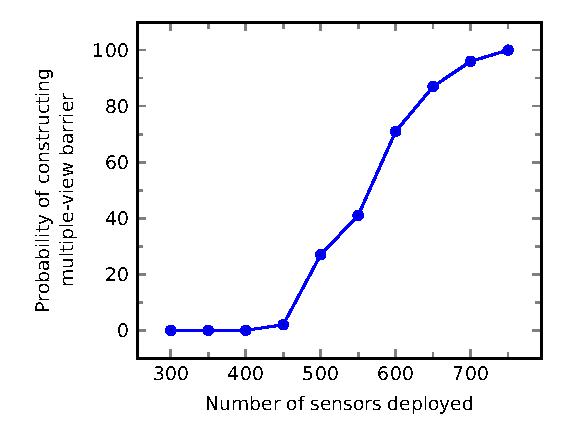
\includegraphics[scale=.8]{Hinhanh/SensorNumberEffect/probability/k3omega105.pdf}
		\caption{k = 3, $\omega$ = 105}
	\end{subfigure}
	\begin{subfigure}{.5\textwidth}
		\centering
		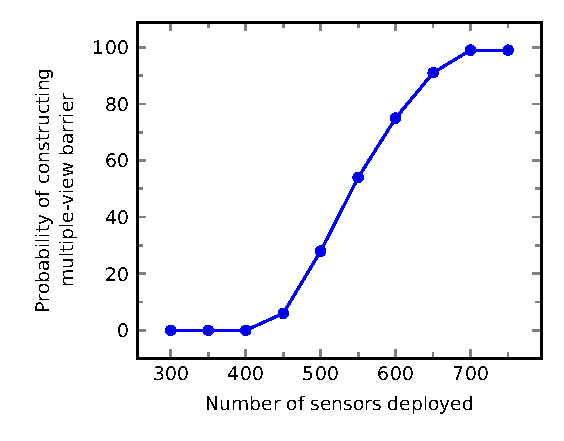
\includegraphics[scale=.8]{Hinhanh/SensorNumberEffect/probability/k4omega65.pdf}
		\caption{k = 4, $\omega$ = 65}
	\end{subfigure}
\caption{Effect of sensor number on the probability of existence of multiple view barrier with some typical values of $k$ and $\omega$}
\label{fig:}
\end{figure}

\subsubsection{Effect of $k$ on algorithm performance}

The parameter $k$ is affected the achieved results the most regarding all 3 aspects. This is because the change in k would manipulate the problem entirely, an answer with a value of $k$ would not be an answer with another value of $k$. As a consequence, the achieved results are drastically different among every value of $k$.

As mentioned in previous parts, generally, the coverage value of the barriers would not be much different from the others. As a result, we may reach a conclusion that for every value of $k$, it is possible to define a critical value of barrier coverage which denotes the largest achieved value of coverage for a certain value of $k$. And this critical coverage value could be use to compare the performance of the problem with different values of $k$.

Regarding this metric, in general, as there are more sensors that cover a certain point, an increase in the value of $k$ may lead to a larger critical coverage value. However, since the function of $cos(x)$ has a derivative getting lower as the value of $x$ comes close to 0, and the effect of increasing $k$ on decreasing the sight angle of sensors to the parts of the intruder ($\phi - \phi_i$) may reduce with larger $k$. As a result, the critical coverage value would rise slower than the rise in the value of $k$.

Finally, the effect of $k$ on computation time is hard to illustrate clearly, since each $k$ would correspond to different values of $\omega$, which makes it impossible to choose which settings of parameters should be compared. However, in general, a greater amount of $k$ would lead to a significant greater computational time. This is because that the large value of $k$ would leads to a larger nest in traversing for all the $k-\omega$ sets and larger loop when checking the coverage value of nodes, hence the computation time for finding all the sets that $k-\omega$ cover each node and determining the sets of sensor with largest coverage value is increased considerably.

\begin{figure}[h]
	\centering
	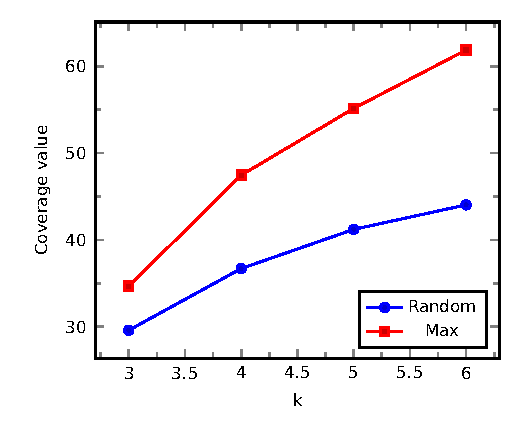
\includegraphics[scale=1.]{Hinhanh/kEffect/main.pdf}
	\caption{Effect of $k$ on the critical coverage value of the $(k-\omega)$ barrier}
	\label{fig:}
\end{figure}

\subsubsection{Experimental conclusion}
Regarding all above analysis, it is possible to achieve some valuable conclusion about the model of $(k-\omega)$.
\begin{itemize}
	\item Firstly, it is notable that the max method overcomes the random method regarding coverage value with a considerable gap between the method results. Despite the surge in computational time due to expensive node handling, the significant offered coverage value prove that it is more suitable to choose the max node handling method.
	\item In terms of model parameters $k$, $\omega$ and sensor number, with the choose of max method, the model offer great result regarding coverage value, computational time and barrier probability with some appropriate settings of parameters.
\end{itemize}